\documentclass{beamer}
\usepackage[utf8]{inputenc}

\usetheme{Madrid}
\usecolortheme{default}
\usepackage{amsmath,amssymb,amsfonts,amsthm}
\usepackage{txfonts}
\usepackage{tkz-euclide}
\usepackage{listings}
\usepackage{adjustbox}
\usepackage{array}
\usepackage{tabularx}
\usepackage{gvv}
\usepackage{lmodern}
\usepackage{circuitikz}
\usepackage{tikz}
\usepackage{graphicx}
\usepackage{mathtools}
\setbeamertemplate{page number in head/foot}[totalframenumber]

\usepackage{tcolorbox}
\tcbuselibrary{minted,breakable,xparse,skins}



\definecolor{bg}{gray}{0.95}
\DeclareTCBListing{mintedbox}{O{}m!O{}}{%
  breakable=true,
  listing engine=minted,
  listing only,
  minted language=#2,
  minted style=default,
  minted options={%
    linenos,
    gobble=0,
    breaklines=true,
    breakafter=,,
    fontsize=\small,
    numbersep=8pt,
    #1},
  boxsep=0pt,
  left skip=0pt,
  right skip=0pt,
  left=25pt,
  right=0pt,
  top=3pt,
  bottom=3pt,
  arc=5pt,
  leftrule=0pt,
  rightrule=0pt,
  bottomrule=2pt,
  toprule=2pt,
  colback=bg,
  colframe=orange!70,
  enhanced,
  overlay={%
    \begin{tcbclipinterior}
    \fill[orange!20!white] (frame.south west) rectangle ([xshift=20pt]frame.north west);
    \end{tcbclipinterior}},
  #3,
}
\lstset{
    language=C,
    basicstyle=\ttfamily\small,
    keywordstyle=\color{blue},
    stringstyle=\color{orange},
    commentstyle=\color{green!60!black},
    numbers=left,
    numberstyle=\tiny\color{gray},
    breaklines=true,
    showstringspaces=false,
}
%This block of code defines the information to appear in the
%Title page
\title %optional
{5.2.61}
%\subtitle{A short story}

\author % (optional)
{Vaishnavi - EE25BTECH11059}



\begin{document}


\frame{\titlepage}
\begin{frame}{Question}
Solve the system:\\
  x - y + 2z = 1 \\
   2z - 3z = 1 \\
  3x - 2y + 4z = 2
\end{frame}
\begin{frame}{allowframebreaks}
\frametitle{Solution}
\begin{table}[H]    
  \centering
  \begin{tabular}{|c|c|}
\hline
\textbf{Name} & \textbf{Value} \\ \hline
$\vec{A}$ & $\myvec{2 & 1 \\0 & 3}$ \\ \hline
\end{tabular}

  \caption{Variables Used}
  \label{tab:1.10.2}
\end{table}

\end{frame}
\begin{frame}{Solution}
 \begin{align}
    \myvec{1 & -1 & 2}\Vec{X}=1\\
     \myvec{0 & 2 & -3}\Vec{X}=1\\
      \myvec{3 & -2 & 4}\Vec{X}=2
\end{align}
\end{frame}


\begin{frame}{Solution}
This system of equations can be solved using an augmented matrix and Gaussian elimination
\begin{align}
&\left(
\begin{array}{ccc|c}
1 & -1 & 2 & 1 \\
0 & 2 & -3 & 1 \\
3 & -2 & 4 & 2
\end{array}
\right)
\xrightarrow{R_3 - 3R_1}
\left(
\begin{array}{ccc|c}
1 & -1 & 2 & 1 \\
0 & 2 & -3 & 1 \\
0 & 1 & -2 & -1
\end{array}
\right) \\
&\xrightarrow{R_3 - \frac{1}{2} R_2}
\left(
\begin{array}{ccc|c}
1 & -1 & 2 & 1 \\
0 & 2 & -3 & 1 \\
0 & 0 & -\frac{1}{2} & -\frac{3}{2}
\end{array}
\right) 
\end{align}
\end{frame}

\begin{frame}{solution}
\begin{align}
&\xrightarrow{R_2 \to \frac{1}{2} R_2}
\left(
\begin{array}{ccc|c}
1 & -1 & 2 & 1 \\
0 & 1 & -\frac{3}{2} & \frac{1}{2} \\
0 & 0 & -\frac{1}{2} & -\frac{3}{2}
\end{array}
\right) \\
&\xrightarrow{R_3 \to -2 R_3}
\left(
\begin{array}{ccc|c}
1 & -1 & 2 & 1 \\
0 & 1 & -\frac{3}{2} & \frac{1}{2} \\
0 & 0 & 1 & 3
\end{array}
\right) \\
&\xrightarrow{R_2 \to R_2 + \frac{3}{2} R_3}
\left(
\begin{array}{ccc|c}
1 & -1 & 2 & 1 \\
0 & 1 & 0 & 5 \\
0 & 0 & 1 & 3
\end{array}
\right) 
\end{align}
\end{frame}
\begin{frame}{Solutions}
\begin{align}
 &\xrightarrow{R_1 \to R_1 - 2 R_3}
\left(
\begin{array}{ccc|c}
1 & -1 & 0 & -5 \\
0 & 1 & 0 & 5 \\
0 & 0 & 1 & 3
\end{array}
\right) \\
&\xrightarrow{R_1 \to R_1 + R_2}
\left(
\begin{array}{ccc|c}
1 & 0 & 0 & 0 \\
0 & 1 & 0 & 5 \\
0 & 0 & 1 & 3
\end{array}
\right) \\
  \Vec{X}=\myvec{0
                    \\
                     5
                    \\
                     3}\\
&x = 0, \quad y = 5, \quad z = 3
\end{align}
\end{frame}








\begin{frame}{Graph}
   Refer to Figure

\begin{figure}[H]
\begin{center}
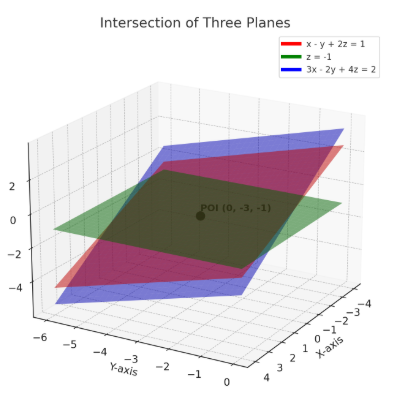
\includegraphics[width=0.6\columnwidth]{../figs/graph9.png}
\end{center}
\caption{}
\label{fig:Fig}
\end{figure}  
\end{frame}




\begin{frame}[fragile]
    \frametitle{Python Code}
    \begin{lstlisting}
import numpy as np
import matplotlib.pyplot as plt
from matplotlib.lines import Line2D

# Intersection point (calculated from the system)
poi = np.array([0, -3, -1])

# Grid for plotting planes
x_range = np.linspace(-4, 4, 30)
y_range = np.linspace(-6, 0, 30)
X, Y = np.meshgrid(x_range, y_range)

# Plane 1: x - y + 2z = 1  ->  z = (1 - x + y) / 2
Z1 = (1 - X + Y) / 2

# Plane 2: z = -1
Z2 = -1 * np.ones_like(X)

# Plane 3: 3x - 2y + 4z = 2  -> z = (2 - 3x + 2y) / 4
Z3 = (2 - 3*X + 2*Y) / 4
\end{lstlisting}
\end{frame}

\begin{frame}[fragile]
    \frametitle{Python Code }

    \begin{lstlisting}
# Create plot
fig = plt.figure(figsize=(10, 8))
ax = fig.add_subplot(111, projection='3d')

# Plot planes with distinct colors
ax.plot_surface(X, Y, Z1, alpha=0.5, color='red')
ax.plot_surface(X, Y, Z2, alpha=0.5, color='green')
ax.plot_surface(X, Y, Z3, alpha=0.5, color='blue')

# Mark and label the intersection point
ax.scatter([poi[0]], [poi[1]], [poi[2]], s=100, c='black', marker='o')
ax.text(poi[0], poi[1], poi[2]+0.3, f'POI (0, -3, -1)', 
        color='black', fontsize=11, weight='bold')

# Labels and title
ax.set_xlabel('X-axis')
ax.set_ylabel('Y-axis')


    \end{lstlisting}
\end{frame}

\begin{frame}[fragile]
    \frametitle{Python Code}

    \begin{lstlisting}
ax.set_zlabel('Z-axis')
ax.set_title('Intersection of Three Planes')

# Add legend manually
legend_elements = [
    Line2D([0], [0], color='red', lw=4, label='x - y + 2z = 1'),
    Line2D([0], [0], color='green', lw=4, label='z = -1'),
    Line2D([0], [0], color='blue', lw=4, label='3x - 2y + 4z = 2')
]
ax.legend(handles=legend_elements, loc='upper right')

# Adjust view angle
ax.view_init(elev=20, azim=30)

# Save the figure
plt.savefig("graph9.png", dpi=300, bbox_inches='tight')
plt.close()



  \end{lstlisting}
\end{frame}

\begin{frame}[fragile]
\frametitle{C Code}
\begin{lstlisting}
#include <stdio.h>

#define N 3  // number of equations

// Function to perform Gaussian elimination
void gaussian_elimination(double A[N][N+1], double x[N]) {
    int i, j, k;

    // Forward elimination
    for (i = 0; i < N-1; i++) {
        for (k = i+1; k < N; k++) {
            double factor = A[k][i] / A[i][i];
            for (j = i; j <= N; j++) {
                A[k][j] -= factor * A[i][j];
            }
        }
    }
          
    \end{lstlisting}

\end{frame}
\begin{frame}[fragile]
\frametitle{C Code}
\begin{lstlisting}
  // Back-substitution
    for (i = N-1; i >= 0; i--) {
        x[i] = A[i][N];
        for (j = i+1; j < N; j++) {
            x[i] -= A[i][j] * x[j];
        }
        x[i] = x[i] / A[i][i];
    }
}

// Exposed function for ctypes
void solve_system(double *solution) {
    // Augmented matrix for given system:
    // x - y + 2z = 1
    // 0x + 2y - 3z = 1
    \end{lstlisting}

\end{frame}

\begin{frame}[fragile]
\frametitle{C Code}
\begin{lstlisting}
  // 3x - 2y + 4z = 2
    double A[N][N+1] = {
        {1, -1,  2, 1},
        {0,  2, -3, 1},
        {3, -2,  4, 2}
    };

    double x[N];
    gaussian_elimination(A, x);

    for (int i = 0; i < N; i++) {
        solution[i] = x[i];
    }
}

\end{lstlisting}
\end{frame}

\begin{frame}[fragile]
\frametitle{Python and C Code}

\begin{lstlisting}
import ctypes

# Load the shared object
lib = ctypes.CDLL("./code.so")

# Define return type and argument type of the exposed function
lib.solve_system.argtypes = [ctypes.POINTER(ctypes.c_double)]
lib.solve_system.restype = None

# Prepare solution array
solution = (ctypes.c_double * 3)()

# Call C function
lib.solve_system(solution)

# Print the result
print("Solution of system:")
print(f"x = {solution[0]}")
print(f"y = {solution[1]}")
print(f"z = {solution[2]}")


\end{lstlisting}

\end{frame}

\end{document}